\section{Theorie}
\label{sec:Theorie}

\subsection{Fehlerrechnung}

Für die Fehlerfortpflanzung bei Gleichungen mit $N$ fehlerbehafteten Größen
wird jeweils die Formel zur Gaußschen Fehlerfortpflanzung

\begin{equation}
  \sigma = \sqrt{\sum_{i=1}^{N}\biggl(\frac{\partial f(x_i)}{\partial x_i}
  \sigma_i\biggr)^2}
\end{equation}
mit der jeweiligen Funktion $f(x_i)$, den Messgrößen $x_i$ und den
zugehörigen Fehlern $\sigma_i$ verwendet.
Zur Berechnung des arithmetischen Mittels von $N$ Messwerten wird jeweils die
Formel

\begin{equation}
  \bar{x} = \frac{1}{N}\sum_{i=1}^{N}x_i
\end{equation}
mit den Messwerten $x_i$ benutzt.
die Standardabweichung des Mittelwerts wird jeweils mit der Gleichung

\begin{equation}
  \bar{\sigma} = \sqrt{\frac{1}{N-1}\sum_{i=1}^{N}(x_i - \bar{x})^2}
\end{equation}
mit den $N$ Messwerten $x_i$ berechnet.

\subsection{Erzeugung von Röntgenstrahlung}

Bei der Erzeugung von Röntgenstrahlung werden Elektronen, die aus einer Glühkathode
austreten, durch eine Beschleunigungsspannung innerhalb einer evakuierten Röhre
auf eine Anode  hin beschleunigt. Die dann entstehende Röntgenstrahlung setzt sich
aus \emph{kontinuierlicher Bremsstrahlung} und \emph{charakteristischer Röntgenstrahlung}
zusammen.

\subsubsection{Die kontinuierliche Bremsstrahlung}

Die beschleunigten freien Elektronen werden vom Coulombfeld der Atome des Anodenmaterials
abgebremst; dabei wird ein Photon ausgesendet, das der Bewegungsenergie des Elektrons
entspricht. Beim Bremsvorgang kann die gesamte oder aber auch nur ein Teil der
kinetischen Energie umgewandelt werden. Deshalb ist das Spektrum kontinuierlich.
Aus der kinetischen Energie \eqref{eqn:Ekin} und der Strahlunsenergie \eqref{eqn:Estrahl}
lässt sich dann berechnen, welche Wellenlänge die abgestrahlten Photonen besitzen, wenn
die gesamte Energie der Elektronen darin umgewandelt werden.

\begin{align}
  E_{\g{kin}} &= \g{e_0} U \label{eqn:Ekin}\\
  E &= \g{h} \nu \label{eqn:Estrahl}
\end{align}

Die Formel zur minimalen Wellenlänge ist dann \eqref{eqn:minlambda}.

\begin{equation}
  \lambda_{\g{min}} = \frac{\g{h} \g{c}}{e_0 U}
  \label{eqn:minlambda}
\end{equation}

\subsubsection{Die charakteristische Röntgenstrahlung}

Die charakteristische Strahlung ist spezifisch für das Anodenmaterial. Sie ensteht,
wenn ein freies beschleunigtes Elektron ein gebundenes Elektron entfernt. Dann
fällt ein Elektron aus einer der höheren Schalen in so entstandene Leerstelle.
Da es von einem höheren Energieniveau in ein niedrigeres übergeht, wird bei dem Vorgang Energie
in Form eines Röntgenquants ausgesendet. Diese Energie ist dann die Energiedifferenz der
beiden Niveaus nach Formel \eqref{eqn:ediff}.

\begin{equation}
  \g{h} \nu = E_{\G{m}}-E_{\G{n}}
  \label{eqn:ediff}
\end{equation}

Da die Niveaus diskrete Werte aufweisen, ist auch die Strahlung diskret und erscheinen
als Linien auf dem Spektrum. Bezeichnet werden sie mit $K_{\g{\alpha}}$, $K_{\g{\beta}}$,
$L_{\g{\alpha}}$ und so weiter.
Hierbei stehen $K, L, M, ...$ für die Schale, in die die Elektronen fallen und
die griechischen Buchstaben stehen für die Herkunft des auffüllenden Elektrons.
$\alpha$ steht also für die nächsthöhere und $\beta$ für die darüber.
Demnach ist die $K_{\g{\alpha}}$-Linie die Emission, die auftritt, wenn ein Elektron
der L-Schale in die K-Schale zurückfällt.

Die Energieniveaus der n-ten Schale werden mit Formel \eqref{eqn:ebind} berechnet.

\begin{equation}
  E_{\g{n}} = -R_{\infty} z_{\g{eff}}^2 \cdot \frac{1}{n^2}
  \label{eqn:ebind}
\end{equation}

Hierbei ist über die \emph{effektive Kernladung} \eqref{eqn:zeff} berücksichtigt, dass
Elektronen auf äußeren Schalen von Elektronen innerer Schalen abgeschirmt werden.
Die Coulomb-Anziehung des Kerns wird also abgeschwächt. Die Rydbergenergie beträgt
$R_{\infty} = \SI{13.6}{\electronvolt}$.

\begin{equation}
  z_{\g{eff}} = z - \sigma
  \label{eqn:zeff}
\end{equation}

Die Abschirmkonstante ist für jedes Elektron unterschiedlich und lässt sich empirisch
bestimmen oder über die Slater-Regeln ermitteln, auf die an dieser Stelle aber nicht
weiter eingegangen werden soll.

Außerdem muss noch erwähnt werden, dass die charakteristischen Linien eine Feinstruktur
aufweisen, weil die äußeren Elektronen durch verschiedene Bahndrehimpulse und Elektronenspins
auch verschiedene Bindungsenergien aufweisen. Die Feinstruktur der $L_{\g{I}}$- und der
$L_{\g{II}}$-Kante können in diesem Versuch nicht nachgewiesen werden; die der $L_{\g{II}}$
und der $L_{\g{III}}$-Kante hingegen schon.

\subsection{Absorption von Röntgenstrahlung}

Der Absorptionskoeffizient nimmt mit steigender Strahlungsenergie für Energien
kleiner als \SI{1}{\mega\electronvolt} gleichmäßig ab. Wenn die
Strahlungsenergie aber gerade die Bindungsenergie eines Elektrons überschreitet, steigt der
Absorptionskoeffizient schlagartig an.
Die Lage der Absorptionskanten wird mit Formel \eqref{eqn:absokant} berechnet. Sie ist nahezu
identisch mit der Bindungsenergie. In Abbildung \ref{fig:absokant} sind diese Kanten
ersichtlich.

\begin{figure}
  \centering
  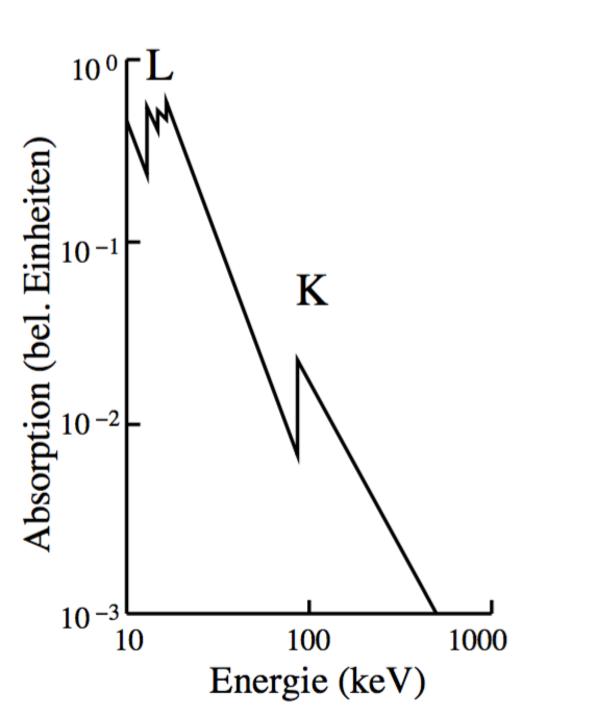
\includegraphics[height = 8cm]{Pics/Absorption.pdf}
  \caption{Der Verlauf des Absorptionskoeffizienten bei zunehmender Energie. \cite{anleitung}}
  \label{fig:absokant}
\end{figure}

Zur Berechnung der Abschirmkonstante $\sigma_{\g{K}}$ kann Formel \eqref{eqn:sigmaK}
verwendet werden.

\begin{align}
  \sigma_{\g{K}} = Z - \sqrt{\frac{E}{R_\infty}- \frac{\alpha^2}{4}z^4}
  \label{eqn:sigmaK}
\end{align}

\begin{equation}
  \g{h} \nu_{\g{abs}} = E_{\g{n}} - E_{\infty}
  \label{eqn:absokant}
\end{equation}

Je nach Lage werden diese Kanten als $K-,L-,M-...Absorptionskante$ bezeichnet.

Die Abschirmkonstante $\sigma_{\g{L}}$ lässt sich mit der Energiedifferenz der $L_{II}$-
und $L_{III}$-Kante bestimmen: $\Delta E_{L} = E_{L_{II}} - E_{L_{III}}$.
Mit Formel \eqref{eqn:sigmal} kann sie dann berechnet werden.

\begin{equation}
  \sigma_{\g{L}} = Z - \left(\frac{4}{\alpha} \sqrt{\frac{\Delta E_{L}}{R_{\infty}}} -
  \frac{5 \Delta E_{L}}{R_{\infty}} \right)^{1/2} \left(1 + \frac{19}{32} \alpha^2 \frac{\Delta E_{L}}{R_{\infty}} \right)^{1/2}
  \label{eqn:sigmal}
\end{equation}

\subsection{Bragg'sche Reflexion}

Zur Beobachtung der Strahlungsenergie muss der Strahl, der aus der Kupfer-Röntgenröhre
austritt aufgefächert werden. Dazu wird er auf ein LiF-Kristallgitter gestrahlt. Dort
werden unterschiedliche Wellenlängen verschieden stark abgelenkt. Die Photonen werden
an jedem Atom des dreidimensionalen Gitters gebeugt und interferieren miteinander.
Konstruktive Interferenz ist beim Glanzwinkel $\theta$ zu erkennen. Er ist gleich
dem Einfallswinkel. In Abbildung \ref{fig:bragg} ist dies zu sehen.

\begin{figure}
  \centering
  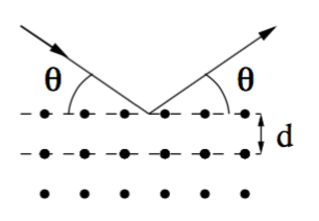
\includegraphics[height = 5cm]{Pics/Bragg.pdf}
  \caption{Die Bragg'sche Reflexion am Gitter. \cite{anleitung}}
  \label{fig:bragg}
\end{figure}

Der Zusammenhang zwischen der Wellenlänge $\lambda$, dem Winkel $\theta$, sowie der
Gitterkonstante $d$ ist in Gleichung \eqref{eqn:braggbed} dargestellt. Hier wurde
stets die erste Beugungsordnung $n=1$ betrachtet.

\begin{equation}
  2 d sin(\theta) = n \lambda
  \label{eqn:braggbed}
\end{equation}
